\chapter{Векторные пространства, базисы и линейные отображения}\label{chap:c26}\markright{Глава 25}
\section{От координат к пространству}
\par\addvspace{5pt}\begin{lrbox}{\CatFlowBox}\begin{minipage}[t]{\linewidth}
\setlength{\parskip}{5pt}\setlength{\columnsep}{4.5mm}\setlength{\intextsep}{0pt}
\begin{wrapfigure}[13]{r}{54mm}

\includegraphics[width=54mm,height=58mm,keepaspectratio]{images/unique/art-102.png}
\end{wrapfigure}
Вектор можно складывать с другим вектором и умножать на число. Эти действия важнее конкретной картинки со стрелками: те же правила выполняются для многочленов и матриц. Абстрактное определение выделяет общие свойства, после чего один аргумент работает сразу во многих примерах. В этой главе поле скаляров \(\mathbb K\) равно \(\mathbb R\) или \(\mathbb C\); если не сказано иное, используем \(\mathbb R\).
\par\WFclear\end{minipage}\end{lrbox}%
\ifdim\dimexpr\ht\CatFlowBox+\dp\CatFlowBox\relax<64mm\dp\CatFlowBox=\dimexpr64mm-\ht\CatFlowBox\relax\fi%
\noindent\usebox{\CatFlowBox}\par\addvspace{5pt}
\begin{definition}
\term{Векторное, или линейное пространство} (\emph{vector space; linear space}) над \(\mathbb K\) — непустое множество \(V\) с операциями \(u+v\in V\) и \(av\in V\), где \(a\in\mathbb K\). Сложение коммутативно и ассоциативно, существует нулевой вектор и у каждого вектора есть противоположный. Кроме того,
\[
\begin{gathered}
a(u+v)=au+av,\qquad (a+b)v=av+bv,\\
a(bv)=(ab)v,\qquad 1v=v.
\end{gathered}
\]
Эти равенства требуются для любых допустимых скаляров и векторов.
\end{definition}
Числа \(a,b\) называют \term{скалярами} (\emph{scalars}). В \(\mathbb R^n\) действия выполняются по координатам. В пространстве \(\mathcal P_m\) элементами служат многочлены \(a_0+a_1t+\dots+a_mt^m\); старшие коэффициенты могут быть нулевыми, поэтому нулевой многочлен включён. Матрицы одного фиксированного размера также образуют пространство при обычном сложении и умножении на скаляр.

\begin{definition}\term{Линейная комбинация} (\emph{linear combination}) векторов \(v_1,\ldots,v_k\) — вектор \(a_1v_1+\dots+a_kv_k\), где \(a_i\in\mathbb K\).\end{definition}
\begin{definition}\term{Линейная оболочка} (\emph{linear span}) \(\operatorname{span}(v_1,\ldots,v_k)\) — множество всех таких комбинаций. Оболочка пустого списка по соглашению равна \(\{0\}\).\end{definition}
\begin{definition}\term{Линейное подпространство} (\emph{linear subspace}) \(W\subseteq V\) — непустое подмножество, замкнутое относительно сложения и умножения на любой скаляр, с операциями, унаследованными от \(V\).\end{definition}
\begin{theorem}[Критерий подпространства]\label{thm:legacy-c26-1}
Непустое \(W\subseteq V\) является подпространством тогда и только тогда, когда \(au+bv\in W\) для всех \(u,v\in W\) и \(a,b\in\mathbb K\).
\end{theorem}
\par\addvspace{5pt}\begin{lrbox}{\CatFlowBox}\begin{minipage}[t]{\linewidth}
\setlength{\parskip}{5pt}\setlength{\columnsep}{4.5mm}\setlength{\intextsep}{0pt}
\begin{wrapfigure}[10]{l}{54mm}
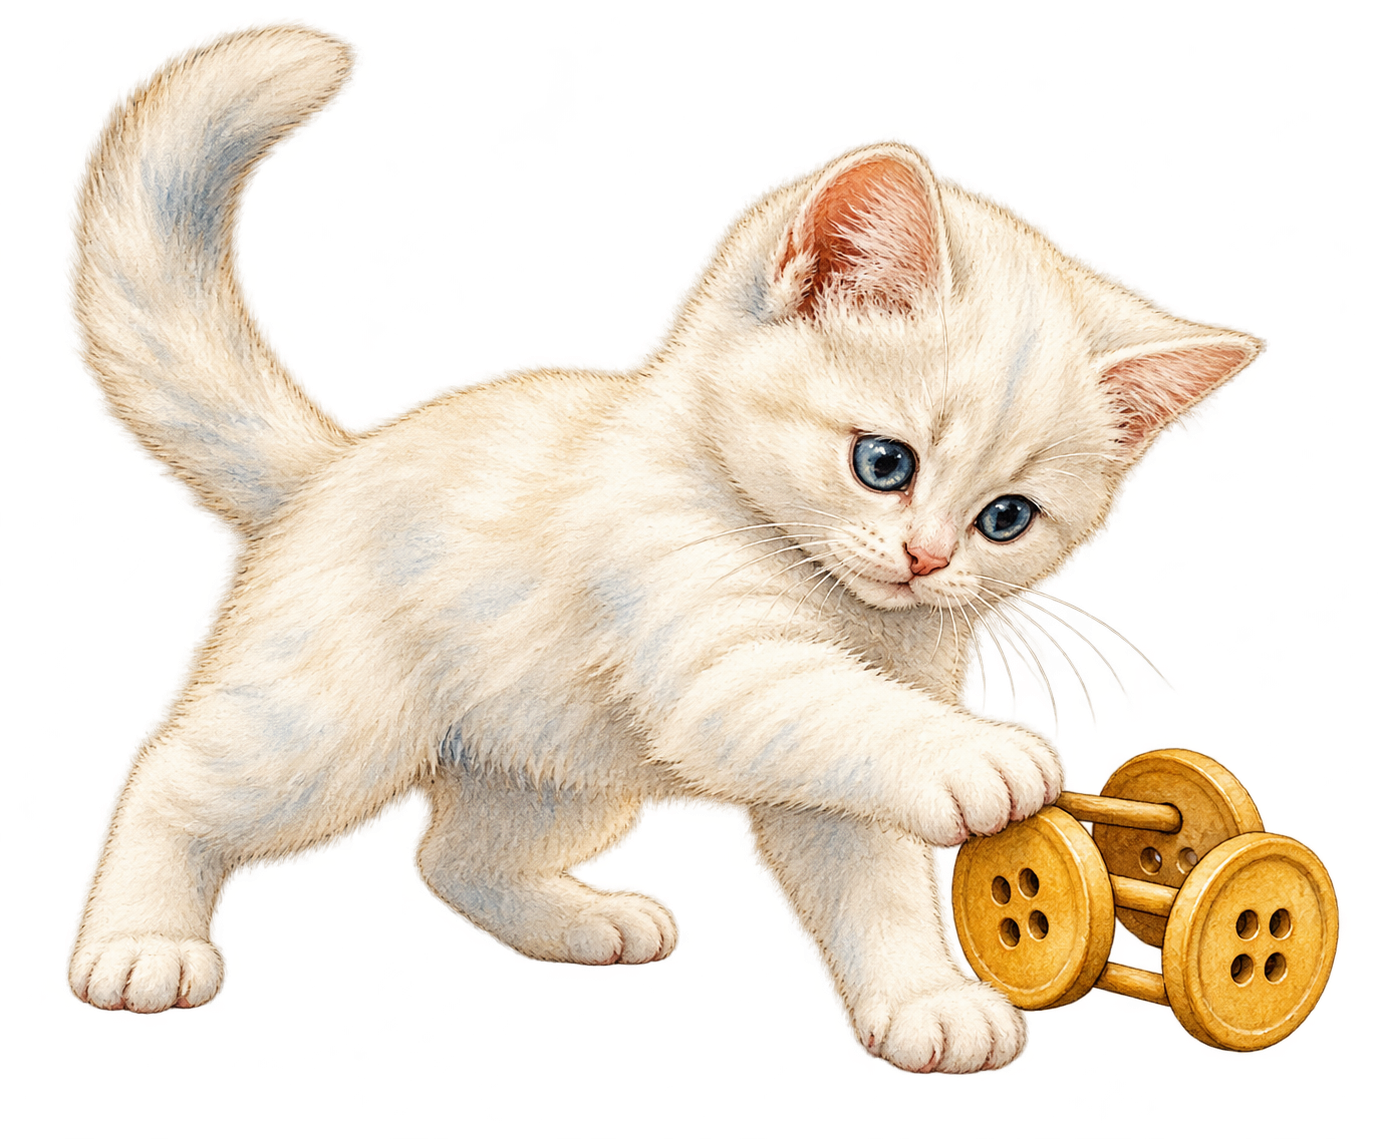
\includegraphics[width=54mm,height=58mm,keepaspectratio]{images/unique/art-105.png}
\end{wrapfigure}
\textit{Доказательство.} Для подпространства это следует из двух замкнутостей. Обратно, выбирая \(a=b=0\), получаем \(0\in W\); выбирая коэффициенты \(1,1\), получаем замкнутость сложения, а \(a,0\) — умножения на скаляр. При \(a=-1\) в \(W\) попадает противоположный вектор. Все остальные аксиомы уже верны в \(V\), поэтому верны и для элементов \(W\).\hfill\(\blacksquare\)
\par\WFclear\end{minipage}\end{lrbox}%
\ifdim\dimexpr\ht\CatFlowBox+\dp\CatFlowBox\relax<64mm\dp\CatFlowBox=\dimexpr64mm-\ht\CatFlowBox\relax\fi%
\noindent\usebox{\CatFlowBox}\par\addvspace{5pt}

Например, решения однородной системы \(Ax=0\) образуют подпространство: \(A(au+bv)=aAu+bAv=0\). Прямая \(x+y=1\) не является подпространством \(\mathbb R^2\), поскольку не содержит нуля. Перенесённая прямая может быть полезным геометрическим объектом, но проверять для неё аксиомы нужно заново.

\section{Независимость, базис и размерность}
\begin{definition}\term{Линейная независимость} (\emph{linear independence}) списка \(v_1,\ldots,v_k\) означает, что равенство \(\sum_{i=1}^ka_iv_i=0\) возможно только при \(a_1=\dots=a_k=0\). Иначе список линейно зависим. Пустой список независим.\end{definition}
\begin{definition}\term{Базис} (\emph{basis}) пространства \(V\) — линейно независимый список векторов, линейная оболочка которого равна \(V\).\end{definition}
\begin{theorem}[Однозначность координат]\label{thm:legacy-c26-2}
Каждый вектор имеет единственное представление линейной комбинацией векторов базиса.
\end{theorem}
\begin{proof}
Существование следует из условия о линейной оболочке. Если две комбинации дают один вектор, вычтем их. Получится нулевая комбинация базисных векторов. Независимость заставляет каждую разность коэффициентов равняться нулю, то есть представления совпадают.
\end{proof}
\begin{definition}\term{Координаты в базисе} (\emph{coordinates relative to a basis}) \(B=(b_1,\ldots,b_n)\) — коэффициенты единственного разложения \(v=\sum a_ib_i\). Их столбец обозначается \([v]_B\).\end{definition}
\par\addvspace{5pt}\begin{lrbox}{\CatFlowBox}\begin{minipage}[t]{\linewidth}
\setlength{\parskip}{5pt}\setlength{\columnsep}{4.5mm}\setlength{\intextsep}{0pt}
\begin{wrapfigure}[9]{l}{54mm}
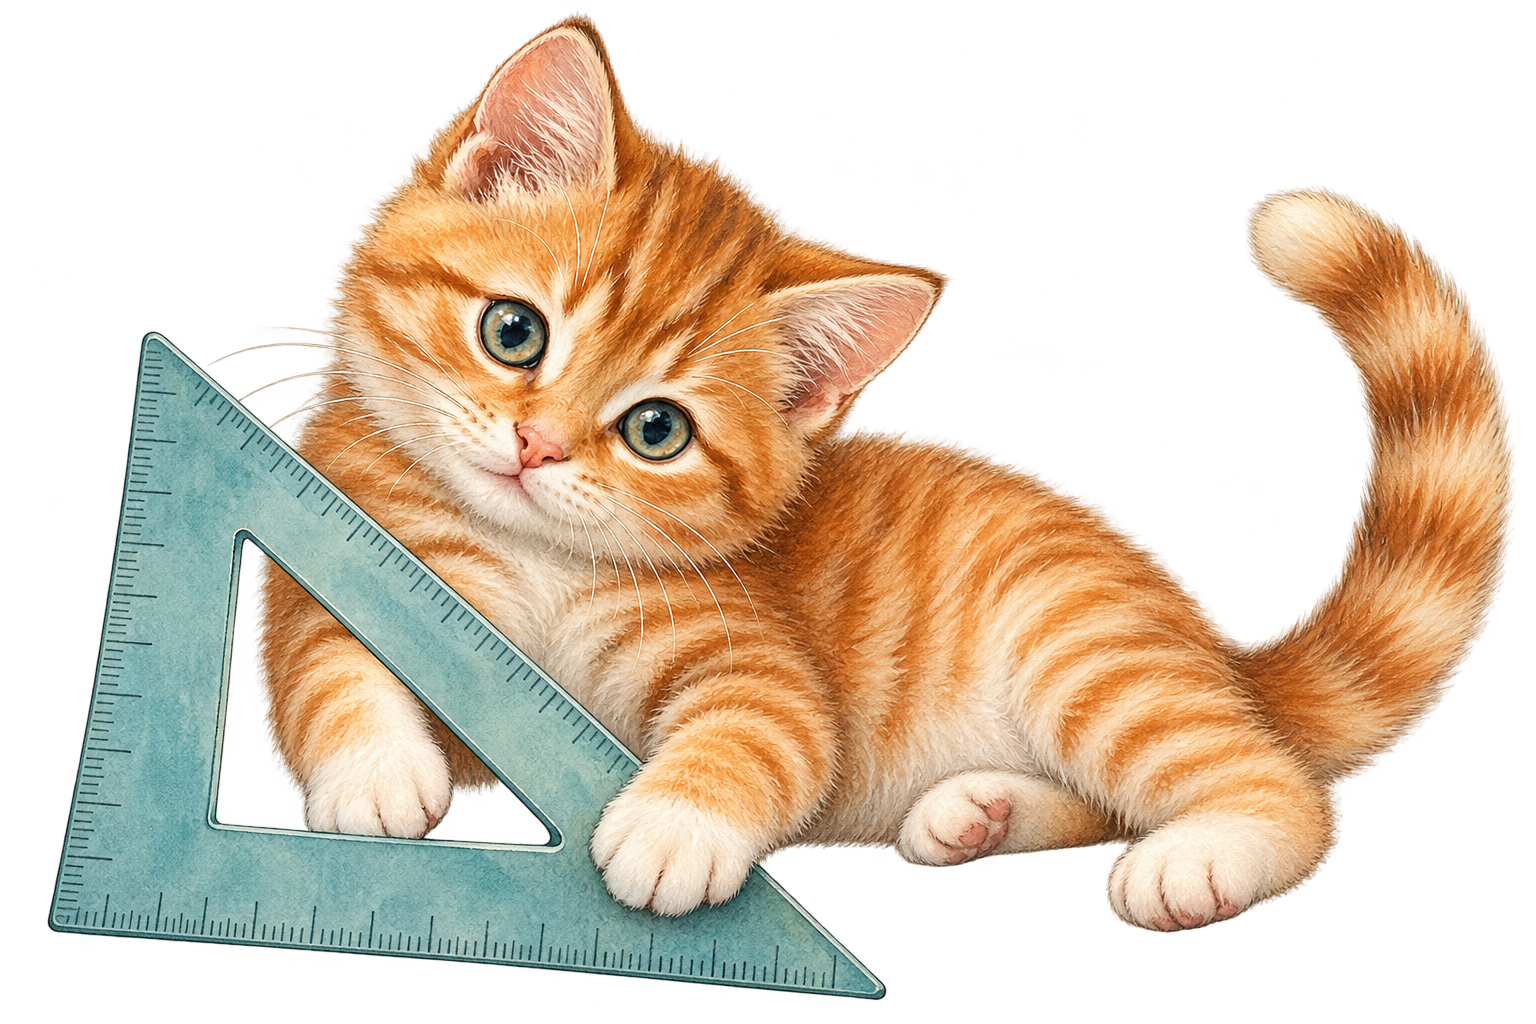
\includegraphics[width=54mm,height=58mm,keepaspectratio]{images/unique/art-103.png}
\end{wrapfigure}
Координаты зависят от выбора базиса, а сам вектор остаётся тем же. Например, \((3,1)=2(1,1)+(1,-1)\), поэтому в базисе \(B=((1,1),(1,-1))\) его координаты равны \((2,1)\), хотя стандартные координаты равны \((3,1)\). Для многочлена роль координат могут играть коэффициенты при \(1,t,t^2\). Наличие удобного базиса превращает вопрос о новых объектах в уже знакомую линейную систему.
\par\WFclear\end{minipage}\end{lrbox}%
\ifdim\dimexpr\ht\CatFlowBox+\dp\CatFlowBox\relax<64mm\dp\CatFlowBox=\dimexpr64mm-\ht\CatFlowBox\relax\fi%
\noindent\usebox{\CatFlowBox}\par\addvspace{5pt}
\begin{theorem}[Конечный базис и число его элементов]\label{thm:legacy-c26-3}
Если \(V\) порождается конечным списком из \(n\) векторов, то у \(V\) есть конечный базис. Любой независимый список содержит не более \(n\) векторов. Все конечные базисы одного пространства имеют одинаковое число элементов.
\end{theorem}
\begin{proof}
Из зависимого порождающего списка можно удалить вектор, выражающийся через остальные: оболочка не изменится. Повторяя удаление, получим независимый порождающий список.

Докажем оценку для независимых \(u_1,\ldots,u_m\) и порождающих \(v_1,\ldots,v_n\). В выражении \(u_1\) через \(v_i\) хотя бы один коэффициент ненулевой; решим равенство относительно соответствующего \(v_i\) и заменим его на \(u_1\). Новый список всё ещё порождает \(V\). После \(k\) замен он содержит \(u_1,\ldots,u_k\). Если есть \(u_{k+1}\), его выражение обязано содержать ненулевой коэффициент при ещё не заменённом \(v_i\), иначе нарушилась бы независимость \(u_j\). Снова выполняем замену. Более \(n\) замен невозможно, значит, \(m\le n\). Для двух базисов применяем эту оценку в обе стороны: их длины равны.
\end{proof}
\begin{definition}\term{Размерность} (\emph{dimension}) конечномерного пространства — число элементов его базиса, обозначаемое \(\dim V\). Для нулевого пространства базис пуст и размерность равна \(0\).\end{definition}
У \(\mathbb R^n\) стандартный базис состоит из \(e_1,\ldots,e_n\), где ровно одна координата равна \(1\). Поэтому \(\dim\mathbb R^n=n\). У \(\mathcal P_m\) базис \((1,t,\ldots,t^m)\), и размерность равна \(m+1\): коэффициенты многочлена определяются однозначно. Пространство всех многочленов без ограничения степени уже не имеет конечного базиса, поскольку конечное число многочленов не порождает степени выше наибольшей из их степеней.

\section{Линейные отображения}
\begin{definition}\term{Линейное отображение} (\emph{linear map; linear transformation}) \(T:V\to W\) над одним полем удовлетворяет \(T(au+bv)=aT(u)+bT(v)\).\end{definition}
\begin{definition}\term{Ядро} (\emph{kernel}) \(T\) — подпространство \(\ker T=\{v:T(v)=0\}\).\end{definition}
\begin{definition}\term{Образ} (\emph{image; range}) \(T\) — подпространство \(\operatorname{im}T=\{T(v):v\in V\}\).\end{definition}
Обе замкнутости следуют из линейности. Выбрав базис в \(V\) и базис в \(W\), получаем матрицу отображения: её столбцы — координаты образов базисных векторов \(V\). Для любого \(v\) линейность даёт \([T(v)]_C=A[v]_B\). Ранг отображения — размерность его образа; для матрицы это совпадает с числом ведущих элементов после метода Гаусса: столбцы исходной матрицы, соответствующие ведущим столбцам ступенчатой матрицы, образуют базис её образа.

\begin{theorem}[Размерность ядра и образа; rank–nullity theorem]\label{thm:legacy-c26-4}
Если \(V\) конечномерно и \(T:V\to W\) линейно, то
\[
\dim V=\dim\ker T+\dim\operatorname{im}T.
\]
В частности, \(T\) инъективно тогда и только тогда, когда \(\ker T=\{0\}\).
\end{theorem}
\begin{proof}
В любом подпространстве можно выбирать независимые векторы, пока они не начнут порождать всё подпространство. Процесс заканчивается не позднее \(\dim V\) шагов по предыдущей теореме. Выберем базис \(u_1,\ldots,u_p\) ядра и дополним его до базиса \(u_1,\ldots,u_p,v_1,\ldots,v_q\) пространства \(V\) тем же способом. Образы \(T(v_j)\) порождают образ, поскольку \(T(u_i)=0\). Если \(\sum c_jT(v_j)=0\), то \(\sum c_jv_j\) лежит в ядре, то есть выражается через \(u_i\). Независимость полного базиса даёт все \(c_j=0\). Значит, образы \(T(v_j)\) — базис образа и \(\dim V=p+q\). Наконец, \(T(u)=T(v)\) равносильно \(T(u-v)=0\), что доказывает критерий инъективности.
\end{proof}

\section{Скалярное произведение в произвольной размерности}
\begin{definition}\term{Евклидово скалярное произведение} (\emph{Euclidean inner product}) в \(\mathbb R^n\) задаётся как \(\langle u,v\rangle=\sum_{i=1}^nu_iv_i\). \par \term{Евклидова норма} (\emph{Euclidean norm}) равна \(\|v\|=\sqrt{\langle v,v\rangle}\).\end{definition}
\begin{definition}\term{Ортогональные векторы} (\emph{orthogonal vectors}) удовлетворяют \(\langle u,v\rangle=0\). Базис называют \par \term{ортонормированным} (\emph{orthonormal}), если его векторы попарно ортогональны и имеют норму \(1\).\end{definition}
\begin{theorem}[Коши–Буняковский в \(\mathbb R^n\)]\label{thm:legacy-c26-5}
Для любых \(u,v\in\mathbb R^n\) выполнено \(|\langle u,v\rangle|\le\|u\|\|v\|\).
\end{theorem}
\begin{proof}
При \(v=0\) обе стороны нулевые. Иначе подставим \(t=\frac{\langle u,v\rangle}{\|v\|^2}\) в неотрицательную сумму \(\|u-tv\|^2\). Раскрытие квадратов даёт \(\|u\|^2-\frac{\langle u,v\rangle^2}{\|v\|^2}\ge0\). Умножение на положительную норму в квадрате и извлечение корня дают результат.
\end{proof}
\par\addvspace{5pt}\begin{lrbox}{\CatFlowBox}\begin{minipage}[t]{\linewidth}
\setlength{\parskip}{5pt}\setlength{\columnsep}{4.5mm}\setlength{\intextsep}{0pt}
\begin{wrapfigure}[12]{r}{54mm}
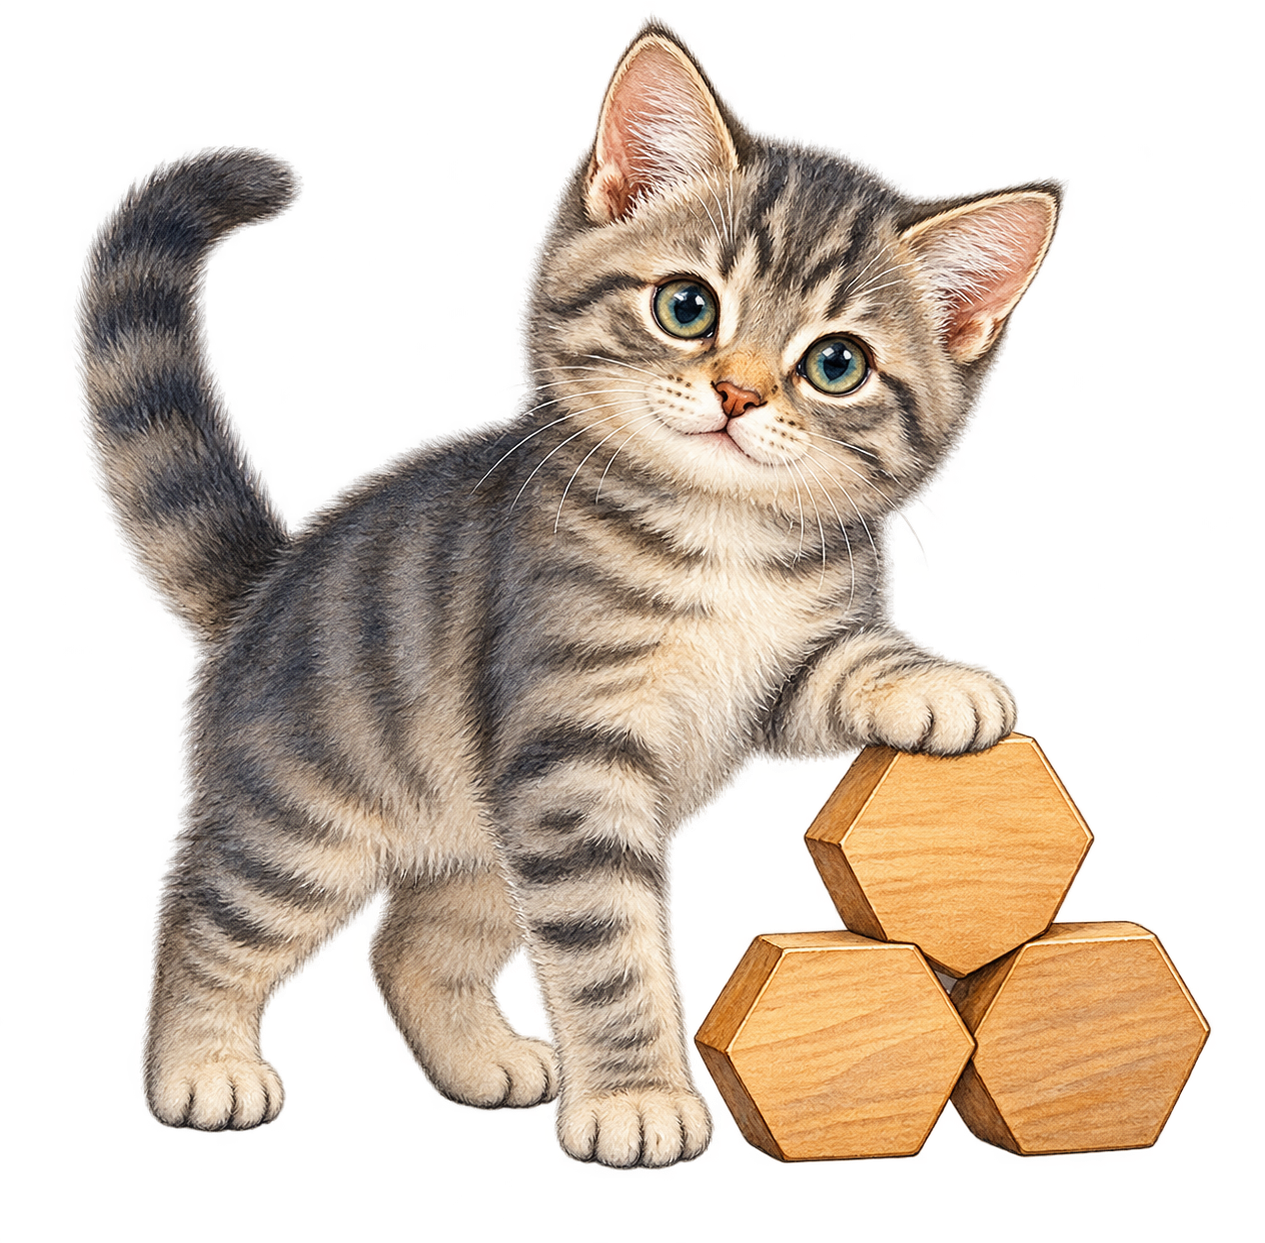
\includegraphics[width=54mm,height=58mm,keepaspectratio]{images/unique/art-104.png}
\end{wrapfigure}
Ортонормированный базис особенно удобен для измерений. Если \(v=\sum a_ib_i\), то \(\langle v,b_j\rangle=a_j\), а \(\|v\|^2=\sum a_i^2\): смешанные произведения исчезают. Поэтому смена одного ортонормированного базиса на другой сохраняет длины. Для произвольного базиса формулу суммы квадратов координат применять без дополнительной проверки нельзя.
\par\WFclear\end{minipage}\end{lrbox}%
\ifdim\dimexpr\ht\CatFlowBox+\dp\CatFlowBox\relax<64mm\dp\CatFlowBox=\dimexpr64mm-\ht\CatFlowBox\relax\fi%
\noindent\usebox{\CatFlowBox}\par\addvspace{5pt}
% END_THEORY_26

\par\noindent\begin{minipage}{\linewidth}\section*{Графики}
\begin{center}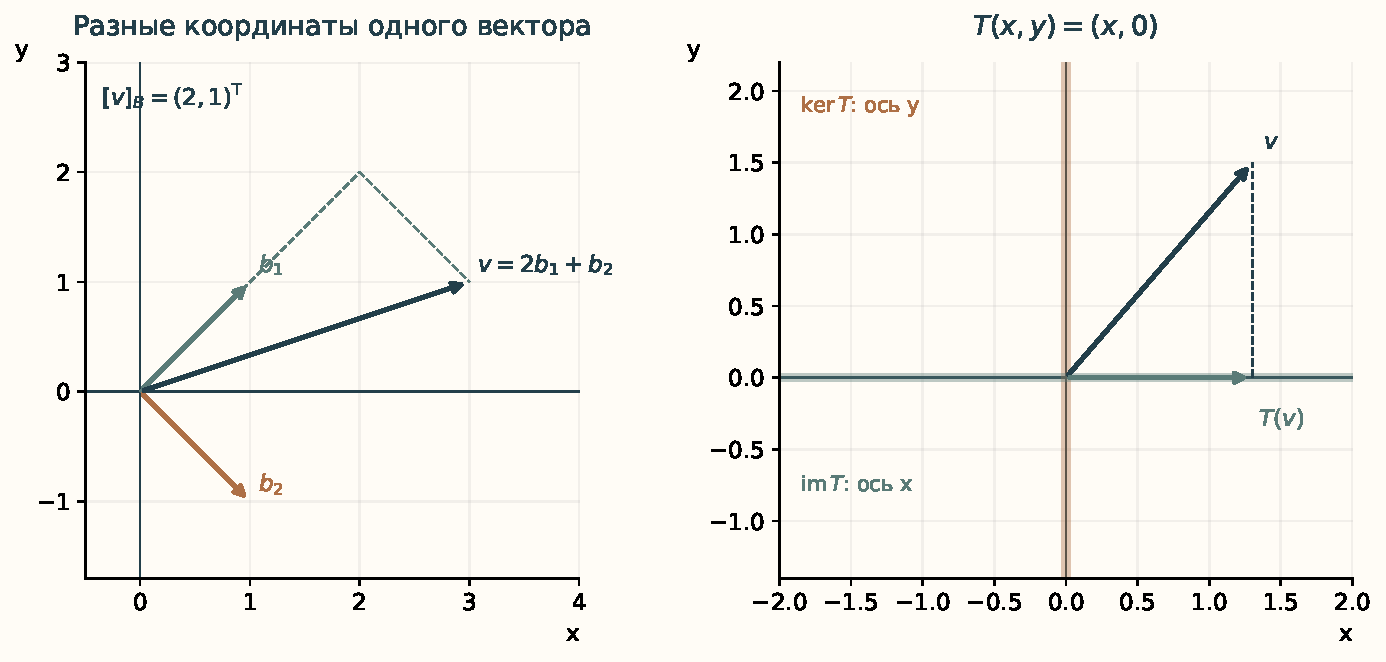
\includegraphics[width=\textwidth,height=.79\textheight,keepaspectratio]{images/atlas-spaces.pdf}\par\small Базис, координаты и ядро\end{center}\end{minipage}\par
\Needspace{7\baselineskip}\section*{Задачи}
\begingroup\setlength{\parskip}{2pt}
\noindent\begin{minipage}[t]{\linewidth}\textbf{25.1.} Проверь, является ли \(W=\{(x,y):x+y=0\}\) подпространством \(\mathbb R^2\). Найди базис.\par\end{minipage}\par
\noindent\begin{minipage}[t]{\linewidth}\textbf{25.2.} Какие из множеств \(x+y=1\), \(y=2x\), \(x\ge0\) являются подпространствами \(\mathbb R^2\)?\par\end{minipage}\par
\noindent\begin{minipage}[t]{\linewidth}\textbf{25.3.} Представь \((5,1)\) через \(u=(1,1)\), \(v=(1,-1)\).\par\end{minipage}\par
\noindent\begin{minipage}[t]{\linewidth}\textbf{25.4.} Независимы ли \((1,2,3)\) и \((2,4,6)\)? Предъяви ненулевые коэффициенты нулевой комбинации.\par\end{minipage}\par
\noindent\begin{minipage}[t]{\linewidth}\textbf{25.5.} Проверь независимость \((1,0,1),(0,1,1),(1,1,0)\) и объясни, образуют ли они базис \(\mathbb R^3\).\par\end{minipage}\par
\par\addvspace{5pt}\begin{lrbox}{\CatFlowBox}\begin{minipage}[t]{\linewidth}
\setlength{\parskip}{5pt}\setlength{\columnsep}{4.5mm}\setlength{\intextsep}{0pt}
\begin{wrapfigure}[11]{r}{54mm}
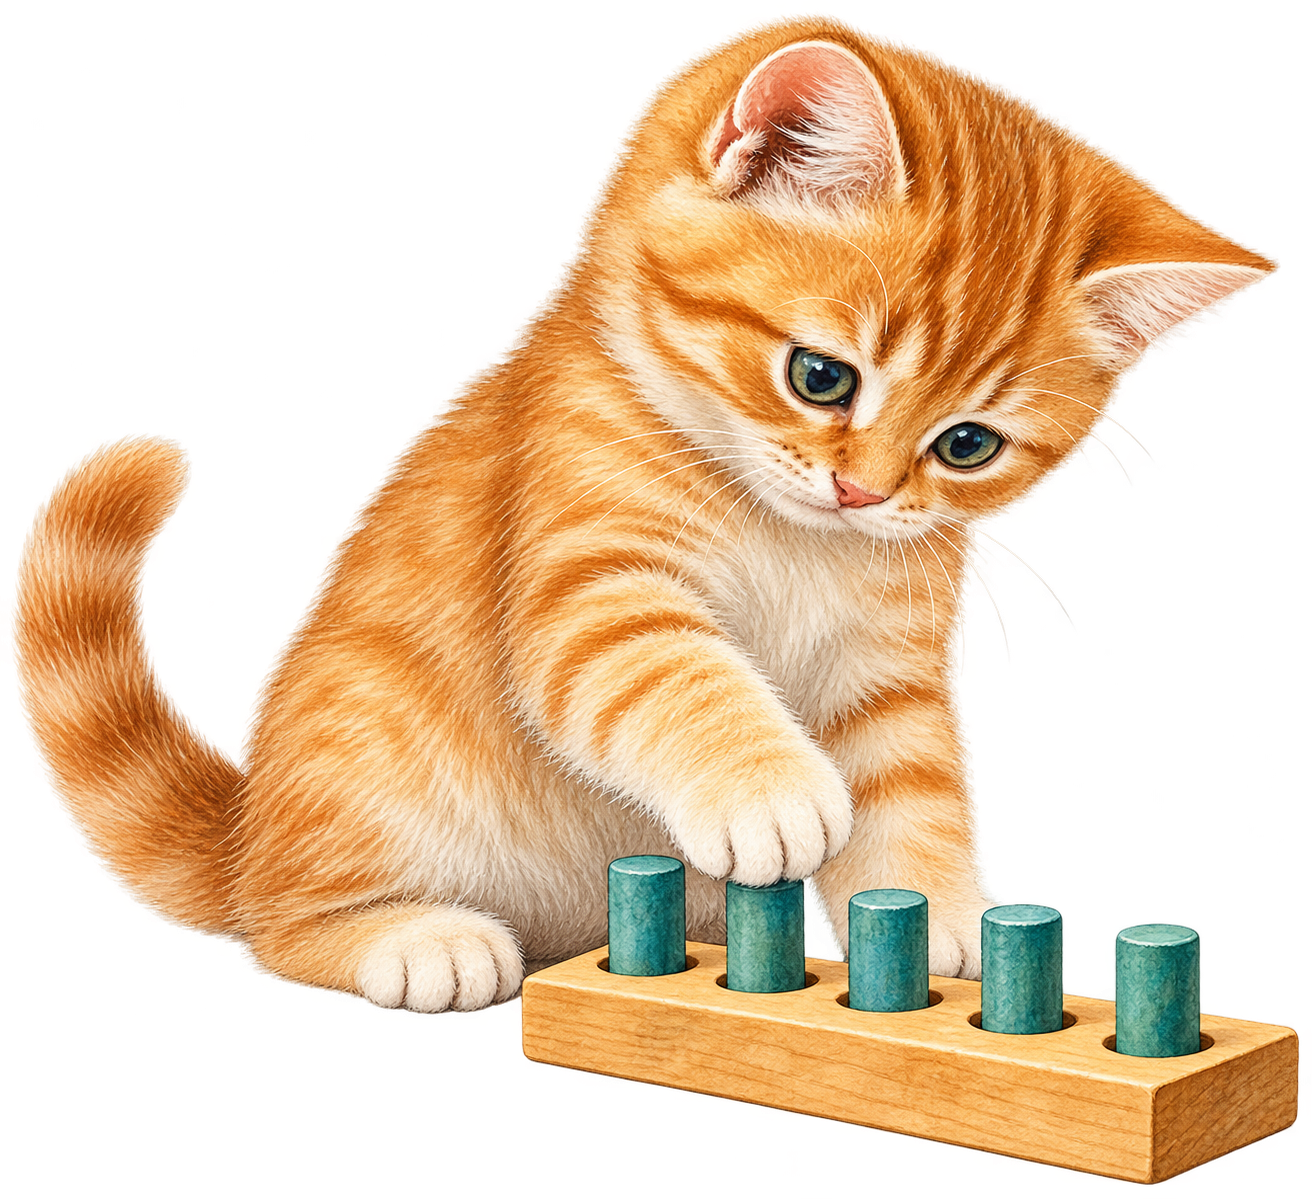
\includegraphics[width=54mm,height=58mm,keepaspectratio]{images/unique/art-106.png}
\end{wrapfigure}
\textbf{25.6.} Найди координаты \((4,-2)\) в базисе \(((1,1),(1,-1))\).\par

\textbf{25.7.} В \(\mathcal P_2\) найди координаты \(3-2t+5t^2\) в базисе \((1,t,t^2)\) и размерность пространства.\par

\textbf{25.8.} Найди базис подпространства многочленов \(p\in\mathcal P_2\), удовлетворяющих \(p(0)=0\).\par

\textbf{25.9.} Какова размерность пространства действительных матриц размера \(2\times3\)? Опиши базис.\par
\par\WFclear\end{minipage}\end{lrbox}%
\ifdim\dimexpr\ht\CatFlowBox+\dp\CatFlowBox\relax<64mm\dp\CatFlowBox=\dimexpr64mm-\ht\CatFlowBox\relax\fi%
\noindent\usebox{\CatFlowBox}\par\addvspace{5pt}

\noindent\begin{minipage}[t]{\linewidth}\textbf{25.10.} Для \(T(x,y,z)=(x+y,y+z)\) найди ядро, образ и их размерности.\par\end{minipage}\par
\noindent\begin{minipage}[t]{\linewidth}\textbf{25.11.} Линейно ли отображение \(T(x,y)=(x+1,y)\)? Обоснуй одним необходимым свойством.\par\end{minipage}\par
\noindent\begin{minipage}[t]{\linewidth}\textbf{25.12.} Линейный датчик выдаёт одно число \(T(x,y,z)=x-2y+z\). Найди два независимых изменения входа, которых датчик не заметит.\par\end{minipage}\par
\noindent\begin{minipage}[t]{\linewidth}\textbf{25.13.} Найди \(\langle u,v\rangle\), \(\|u\|\), \(\|v\|\) для \(u=(1,2,-1)\), \(v=(2,0,2)\). Ортогональны ли векторы?\par\end{minipage}\par
\noindent\begin{minipage}[t]{\linewidth}\textbf{25.14.} Нормируй \((3,4,0)\). Сколько единичных векторов лежит на той же прямой?\par\end{minipage}\par
\noindent\begin{minipage}[t]{\linewidth}\textbf{25.15.} Докажи, что пересечение двух подпространств является подпространством.\par\end{minipage}\par
\noindent\begin{minipage}[t]{\linewidth}\textbf{25.16.} Приведи два подпространства \(\mathbb R^2\), объединение которых не является подпространством.\par\end{minipage}\par
\noindent\begin{minipage}[t]{\linewidth}\textbf{25.17.} Докажи: список, содержащий нулевой вектор, зависим. Что меняется для пустого списка?\par\end{minipage}\par
\noindent\begin{minipage}[t]{\linewidth}\textbf{25.18.} Линейное отображение \(T:\mathbb R^4\to\mathbb R^3\) имеет ранг \(2\). Найди размерность ядра. Может ли оно быть инъективным?\par\end{minipage}\par
\noindent\begin{minipage}[t]{\linewidth}\textbf{25.19.}\starmark{} Докажи, что любые пять векторов \(\mathcal P_3\) линейно зависимы.\par\end{minipage}\par
\noindent\begin{minipage}[t]{\linewidth}\textbf{25.20.}\starmark{} Пусть \(D:\mathcal P_3\to\mathcal P_2\) задано формулой \(D(a_0+a_1t+a_2t^2+a_3t^3)=a_1+2a_2t+3a_3t^2\). Докажи линейность, найди ядро и образ. Позже этот оператор будет называться производной многочлена.\par\end{minipage}\par
\noindent\begin{minipage}[t]{\linewidth}\textbf{25.21.} В ортонормированном базисе \(b_1,b_2\) сила имеет вид \(F=6b_1+8b_2\). Найди длину и проекции на обе оси.\par\end{minipage}\par
\noindent\begin{minipage}[t]{\linewidth}\textbf{25.22.}\starmark{} Докажи, что линейное отображение между двумя пространствами одинаковой конечной размерности инъективно тогда и только тогда, когда сюръективно.\par\end{minipage}\par
\endgroup
